

\subsection{Web application implementation and user
interface}

We built the application using several technologies
where each communicates with each other to provide a
user-friendly website for the potential tourist.
Figure~\ref{TechStack} shows the tech stack diagram of the website.
The website is accessible through the URL
\url{https://www.touristplanner.xyz}. We built the front end of the website using HTML, CSS and javascript and hosted it
on a cloud Vultr server. The website is 
responsive to be accessible from both a
mobile phone and a laptop. The website communicates
with the back end of the application using REST
endpoints, hosted on a separate dedicated server
provided and developed the Java Spring Boot
framework.  Another Python Gunicorn server is used to
generate the itinerary and calculate a travel interest
vector which sends the information directly to the
Spring boot server. Finally, a local instance of an
Open Source Routing Machine server calculates the
distances from one tourist attraction to another used
by the Gunicorn server to optimise the itinerary. 

\begin{figure}[h]
\centering
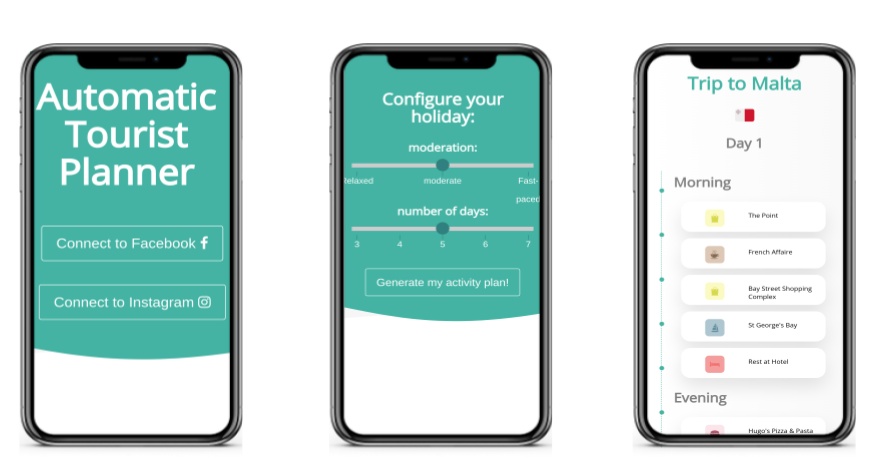
\includegraphics[width=1\textwidth]{Process.png}
\caption{User Experience Timeline}
\label{Timeline}
\end{figure}

Figure~\ref{Timeline} shows screenshots of the website portraying
the user's timeline.  The user navigates to the
homepage, accepts terms and conditions and connect his
social media profiles.  The user selects the number of
days M and the activity activity pace C.  The website
navigates to the final page of the application
exhibiting their personalised itinerary. 
